% !TEX root = main.tex
%%%%%%%%%%%%%%%%%%%%%%%%%%%%%%%%%%%%%%%%
%%%%%%%%%%%%%%%%%%%%%%%%%%%%%%%%%%%%%%%%
\section{Results Discussion} \label{sec:results}
%%%%%%%%%%%%%%%%%%%%%%%%%%%%%%%%%%%%%%%%
%%%%%%%%%%%%%%%%%%%%%%%%%%%%%%%%%%%%%%%%

We discuss the achieved results by research question.


\subsubsection{RQ$_{1}$: Injecting a single log statement}
\label{sec:rq1}

\tabref{tab:single-train-results} reports the results achieved by \approach and LANCE, in terms of correct and partially correct predictions for the task of single-log injection. For \approach we only report the results when $k=5$, since this is the variant that achieved the best performance (results with $k=1$ and $k=3$ are available in \cite{replication}). The first row of \tabref{tab:single-train-results} shows the percentage of correct predictions by both approaches, which is slightly higher for \approach (+1.8\% of relative improvement, from 26.78\% to 27.26\%). This difference is statistically significant (adj. $p$-value $<$ 0.01) with 1.12 higher odds of obtaining a correct prediction from \approach as compared to LANCE. 

\begin{table}[h!]
  \centering
  \caption{Correct predictions considering the four-dimensional challenges of injecting log statements.}
  \resizebox{.5\textwidth}{!}{
	  \begin{tabular}{cccccrrrr}
	  \hline
	  Variable   & Level     & Message   & Position  &  & \multicolumn{1}{c}{LEONID} & \multicolumn{1}{c}{LANCE} & \multicolumn{1}{c}{$p$-value} & \multicolumn{1}{c}{OR}     \\ \hline
	  \ding{51}  & \ding{51} & \ding{51} & \ding{51} &  & 27.26\%                    & 26.78\%                   &                           &                            \\
	  \ding{51}  & -         & -         & -         &  & 76.45\%                    & 77.15\%                   &                           &                            \\ 
	  -          & \ding{51} & -         & -         &  & 73.53\%                    & 74.18\%                   &                           &                            \\
	  -          & -         & \ding{51} & -         &  & 31.55\%                    & 30.16\%                   &                           &                            \\ 
	  -          & -         & -         & \ding{51} &  & 82.35\%                    & 82.28\%                   &                           &                            \\ \hline
	  \ding{51}  & \ding{51} & \ding{55} & \ding{51} &  & 28.14\%                    & 29.86\%                    &                           &                            \\ \hline 
	  
	  \end{tabular}
  }
  \label{tab:single-train-results}
\end{table}




The four subsequent rows report the cases in which one of the four log-statement components (variable, level, message, and position) was correctly predicted (\cmark), independently from whether the other three components were correct or not ($-$). As it can be seen, there is no significant difference in the prediction of the log position, with both techniques correctly predicting it in $\sim$82.3\% of cases. Differences are observed for the log variable and level in favor of LANCE (+1.0\% and +0.9\% relative improvement), and for the log message in favor of \approach (+4.6\% relative improvement). The log message is the part for which we observed the strongest OR among all comparisons. Considering that the only difference between \approach and LANCE is the usage of IR, the improvement in the generation of meaningful log messages we targeted has been at least partially achieved. The latter has, however, a small price to pay in the correct prediction of the log variable and level. Still, for these elements \approach is able to generate a correct prediction in over 73.5\% of cases, while the correct generation of the log message still represents the Achilles' heel of these techniques, with 31.55\% correct predictions achieved by \approach. Thus, we believe that improvements on the log message predictions should be favored even at the expense of losing a bit of prediction capabilities on other elements. 

Digging further into the quality of the generated log messages, \tabref{tab:log-messages-stats} reports the results computed using the four NLP metrics presented in \secref{sec:design} for both models (in bold the best results). All metrics suggest that the log messages generated by \approach are closer to those written by humans. According to our statistical analysis (results in \cite{replication}), all these differences are statistically significant (adj. $p$-value $<$ 0.001) with, however, a negligible effect size. For instance, in a recent study Roy \etal \cite{metricsImprovement} showed that differences in METEOR score lower than 2 points are difficult to perceive for humans. 

In our case, we achieved a 1.75 difference. Thus, while overall our analysis showed some improvement in the log message generation when moving from LANCE to \approach, it is unclear whether this has a practical effect when these tools are used by humans.

\begin{table}[h]
	\vspace{-0.2cm}
	\centering
	\caption{RQ$_1$: Evaluation Metrics on Log Messages: LEONID \emph{vs} LANCE\vspace{-0.3cm}}
	\scriptsize
	\label{tab:log-messages-stats}
	 %\resizebox{.5\textwidth}{!}{
	\begin{tabular}{lrr}
		\toprule
		& {\bf LANCE}  &  {\bf LEONID ($k=5$)} \\\midrule
		BLEU-A \cite{papineni2002bleu}& 31.98 & \bf 35.36\\
			\hspace{0.2cm} BLEU-1 & 47.30  & \bf 50.00\\
			\hspace{0.2cm} BLEU-2 & 36.30  & \bf 39.60\\
			\hspace{0.2cm} BLEU-3 & 33.90  & \bf 35.00\\
			\hspace{0.2cm} BLEU-4 & 31.40  & \bf 32.40\\
		METEOR \cite{meteor} & 58.60  & \bf 60.35 \\
		ROUGE-LCS \cite{lin2004rouge} &  \\
		\hspace{0.2cm} $precision$ & 42.57 & \bf 44.68\\
		\hspace{0.2cm} $recall$ & 44.04 &   \bf 46.01\\
		\hspace{0.2cm} $fmeasure$ & 42.19 &  \bf 44.33\\
		LEVENSHTEIN \cite{levenshtein1966} & 44.02 & \bf 41.85 \\\bottomrule
	\end{tabular} 
	\vspace{-0.2cm}
%}
\end{table}


Also the result of our manual inspection of 300 partially correct predictions by \approach and by LANCE point to a similar story: We found 198 of those generated by \approach (66\%) to report the same information of the target log message, despite being semantically different. The remaining 102 (34\%) predictions, instead, reported a log message completely different from the target one or not meaningful at all. For LANCE, the number of semantically equivalent log messages is slightly lower --- 192 (64\%) --- but inline with that observed for \approach. Examples of different but semantically equivalent log messages generated by \approach are available in our replication package \cite{replication}.


\vspace{0.2cm}
\begin{resultbox}
\textbf{Answer to RQ$_1$.} The 3.6 larger training dataset (as compared to the one by Mastropaolo \etal \cite{mastropaolo2022using}) we used to reproduce LANCE, resulted in a boost of performance when predicting the log message (15.20\% in \cite{mastropaolo2022using} \emph{vs} 30.16\%). Such a result has been further improved by \approach, which achieves a +4.6\% relative improvement (\ie 31.55\% of correctly generated log messages). All metrics used to assess the quality of the log messages generated by \approach indicate improvements over LANCE. However, these improvements are marginal, showing that more research is needed to further improve the automated generation of log messages.
\end{resultbox}




%if we have space put this back
%\begin{figure*}[h]
%	\centering
%	\label{fig:rq1-message-stats}
%	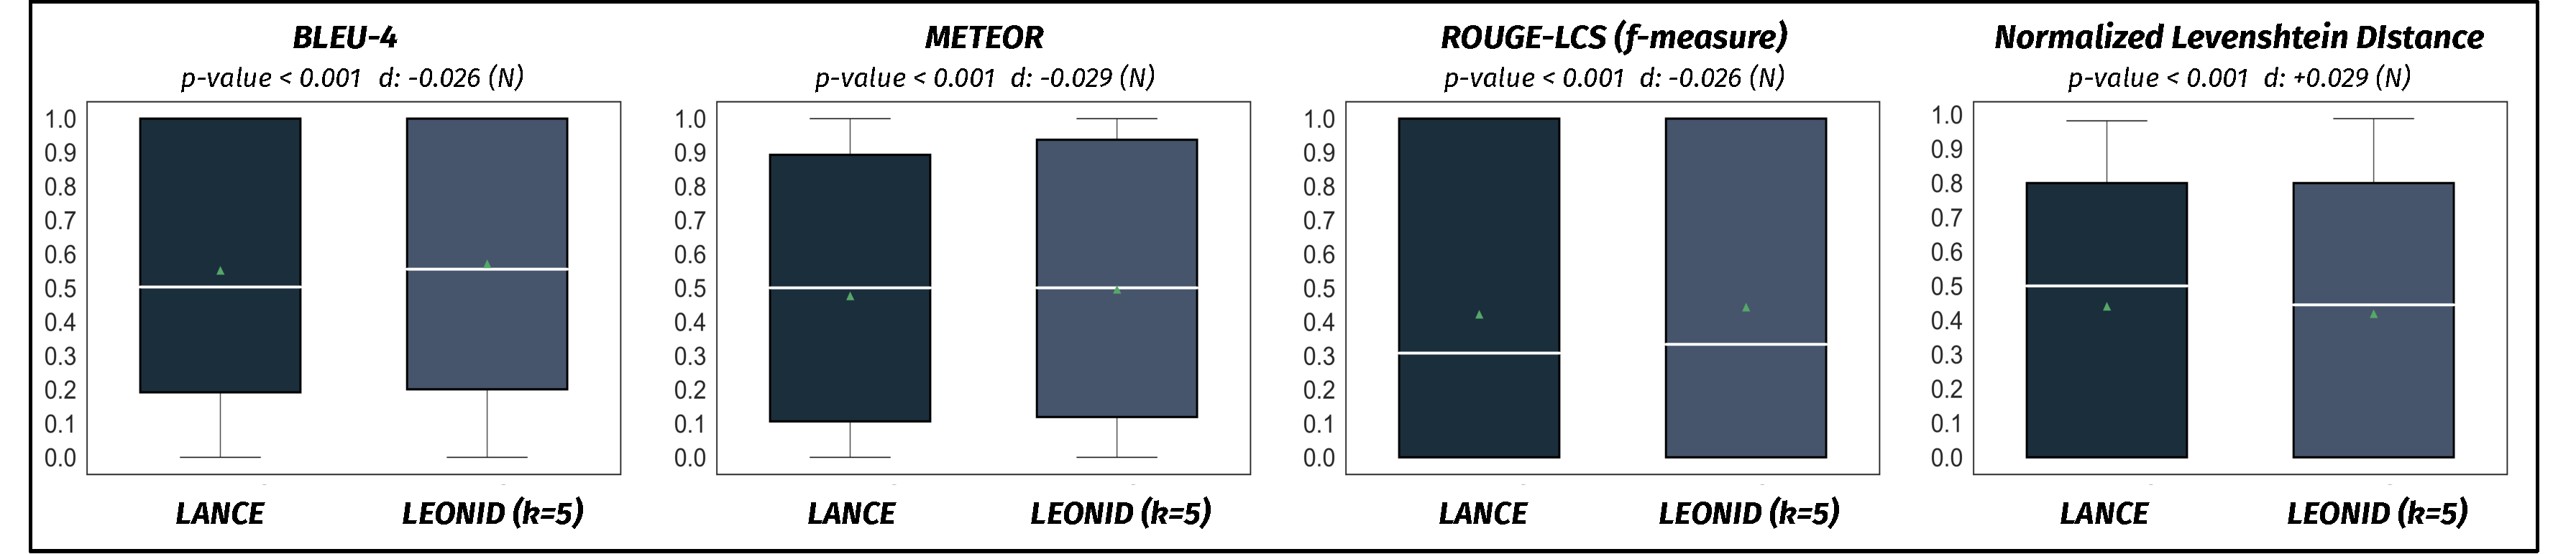
\includegraphics[width=\textwidth]{img/RQ1-log-message-boxplot.pdf}
%	\caption{Characteristics of log messages synthesized by LANCE and LEONID (K=5)}
%\end{figure*}








%\begin{table}[ht]
%	\centering
%	\caption{RQ$_1$: Statistical Tests: LEONID \emph{vs} LANCE for NLP metrics\vspace{-0.3cm}}
%	\scriptsize
%	\label{tab:test-wilcoxon}
%	 \resizebox{.5\textwidth}{!}{
%	\begin{tabular}{llrc}
%		\toprule
%		\textbf{Comparison} & \textbf{Metric} & \textbf{\emph{p}-value} & \textbf{d} \\ 
%		\midrule
%%		\multirow{3}{*}{LANCE  \emph{vs} LEONID ($k=1$)} & BLEU-4 & $<$0.001 & -0.022 (N) \\ 
%%			& METEOR & $<$0.001 & -0.025 (N) \\
%%		& ROUGE-LCS (f-measure) & $<$0.001 & -0.025 (N) \\ 
%%		& LEVENSHTEIN & $<$0.001 & +0.023 (N) \\\midrule
%%		\multirow{3}{*}{LANCE  \emph{vs} LEONID ($k=3$)} & BLEU-4 & $<$0.001 & -0.026 (N) \\ 
%%		& METEOR & $<$0.001 & -0.029 (N) \\
%%		& ROUGE-LCS (f-measure) & $<$0.001 & -0.023 (N) \\ 
%%		& LEVENSHTEIN & $<$0.001 & +0.027 (N) \\\midrule
%			\multirow{4}{*}{LANCE  \emph{vs} LEONID ($k=5$)} & BLEU-4 & $<$0.001 & -0.026 (N) \\ 
%		& METEOR & $<$0.001 & -0.029 (N) \\
%		& ROUGE-LCS (f-measure) & $<$0.001 & -0.026 (N) \\ 
%		& LEVENSHTEIN & $<$0.001 & +0.029 (N) \\\midrule
%	\end{tabular}
%}
%	\vspace{-0.2cm}
%\end{table}


\subsubsection{Performance of LEONID in injection multiple complete log statements in \java methods (RQ$_{2}$)}
\label{sec:rq2}
As explained in \secref{sec:design}, for RQ$_{2}$ we would not be able to compute the partially correct predictions as we performed for RQ$_{1}$. For such a reason, we limit our discussion presenting the results achieved by LEONID when injecting multiple log statements in \java Methods, while reporting qualitative examples in our online appendix \cite{}. To this extent, we found out LEONID to correctly inject multiple log statements in \java methods in 23.38\% (5,634 out of 24,088) when using a ``shallow'' coding context $k=1$. Similarly, even when increasing the window of the coding context (\ie $k=3$ and $k=5$), the achieved results do not undergo major changes, with 23.35\% for $k=3$ and 23.51\% for $k=5$.


\subsubsection{Performance of LEONID in properly deciding whether or not a \java method needs log statements  (RQ$_{3}$)}
\label{sec:rq3}

\figref{fig:rq3-cm} reports the confusion matrices with their respective values of accuracy, precision and recall (on the bottom of the figure) for each test-set in \tabref{tab:ds-summary-2}.

When half of the methods need at least one log statement, and the other half do not need any (50-50 split), LEONID reports an accuracy of 0.96 while achieving a precision of 0.98 and a recall of 0.94. In contrast the \textit{optimistic} and \textit{pessimistic} classifier would achieve 0.50 of accuracy and precision, while reporting a recall of 1.0. 
The \textit{random} classifier on the same test-set (50-50), achieves 0.50 of accuracy, precision, and recall (as expected). 

When testing LEONID on the 75-25 split, there is a slightly increase in terms of precision as compared to the 50-50 split, 0.98 \emph{vs} 0.99. Consequently, the accuracy loose 0.01 points (0.95) as compared to the previous 50-50 split. Instead, the recall keeps its value fixed at 0.94.
The \textit{optimistic} classifier reports a value of 0.75 for both accuracy and precision, while achieving a recall of 1.0. As expected, the \textit{pessimistic} classifier achieves 0.25 points for both accuracy and precision and, 1.0 of recall. As for the \textit{random} classifier, we found out an accuracy and a recall of 0.5, with a precision of 0.75.

When LEONID is tested in a scenario where the number of methods requiring log statements is outweighed by the number of methods that do not need log statements (25-75 split), precision and recall achieve both 0.94. The accuracy for such a scenario is 0.97. 
On the other hand, the \textit{optimistic} classifier would achieve a recall of 1.0, with accuracy and precision both of 0.25, which contrasts the results achieved with the \textit{pessimistic} classifier, which would report a recall of 1.0,  with accuracy and precision of 0.75. On such dataset, the \textit{random} classifier would ensure a precision of 0.25, with accuracy and recall of 0.50.

Finally, as for the test-set resembling the original distribution of \java methods we mined (2-98 split), LEONID achieves an accuracy of 0.98 and a recall of 0.96. Instead, the precision goes down to 0.51.
As for the naive classifiers, we found out that when using the \textit{optimistic}, the achieved accuracy and precision would be both 0.02 points, with a recall of 1.0.
In contrast, the \textit{pessimistic} performs better than LEONID (as expected), achieving 0.97 for both accuracy and precision, and 1.0 for recall.
The \textit{random} classifier, on the other hand, would ensure accuracy of 0.50, and a recall of 0.53, while achieving only 0.02 of precision.


\begin{table}[ht]
	\centering
	\caption{Statistical Tests: LEONID \emph{vs} NAIVE Classifiers\vspace{-0.2cm}}
	\scriptsize
	\label{tab:statistical-classifier}
	\resizebox{.5\textwidth}{!}{
		\begin{tabular}{llrc}
			\toprule
			\textbf{Test Set} & \textbf{Metric} & \textbf{\emph{p}-value} & \textbf{OR} \\ 
			\midrule
			\multirow{3}{*}{Need4Log: (50-50)} 
			& Optimistic \emph{vs} LEONID & $<$0.001 &18.57 \\ 
			& Pessimistic \emph{vs} LEONID & $<$0.001 & 50.28 \\ 
			& Random \emph{vs} LEONID & $<$0.001 & 27.12 \\\midrule
			\multirow{3}{*}{Need4Log: (75-25)} 
			& Optimistic \emph{vs} LEONID & $<$0.001 & 6.17 \\ 
			& Pessimistic \emph{vs} LEONID & $<$0.001 & 140.43 \\ 
			& Random \emph{vs} LEONID & $<$0.001 & 21.41 \\\midrule
			\multirow{3}{*}{Need4Log: (25-75)} 
			& Optimistic \emph{vs} LEONID & $<$0.001 & 54.58 \\ 
			& Pessimistic \emph{vs} LEONID & $<$0.001 & 16.73 \\ 
			& Random \emph{vs} LEONID & $<$0.001 & 33.77 \\\midrule
			\multirow{3}{*}{Need4Log: (2-98)} 
			& Optimistic \emph{vs} LEONID & $<$0.001 & 1,426 \\ 
			& Pessimistic \emph{vs} LEONID & 0.63 & 1.05 \\ 
			& Random \emph{vs} LEONID & $<$0.001 & 56.53 \\\midrule
		\end{tabular}
	}
	\vspace{-0.2cm}
\end{table}


The results of the statistical comparison made using McNemar’s test are reported in \tabref{tab:statistical-classifier}.
As it is shown, LEONID has a positive (OR$>$1) and statistically significant effect in all cases but one. When testing LEONID against the Need4Log (2-98) dataset, we found that for the comparison \textit{Pessimistic} \emph{vs} LEONID, although the OR$>$1, the $p$-value of 0.63 points out to a non statistically significant effect. Such a results is indeed expected, seen the distribution of the labels (\ie \textit{Need}, \textit{No need}) featuring the Need4Log (2-98) dataset. 


\begin{figure*}[h!]
	\centering
	\label{fig:rq3-cm}
	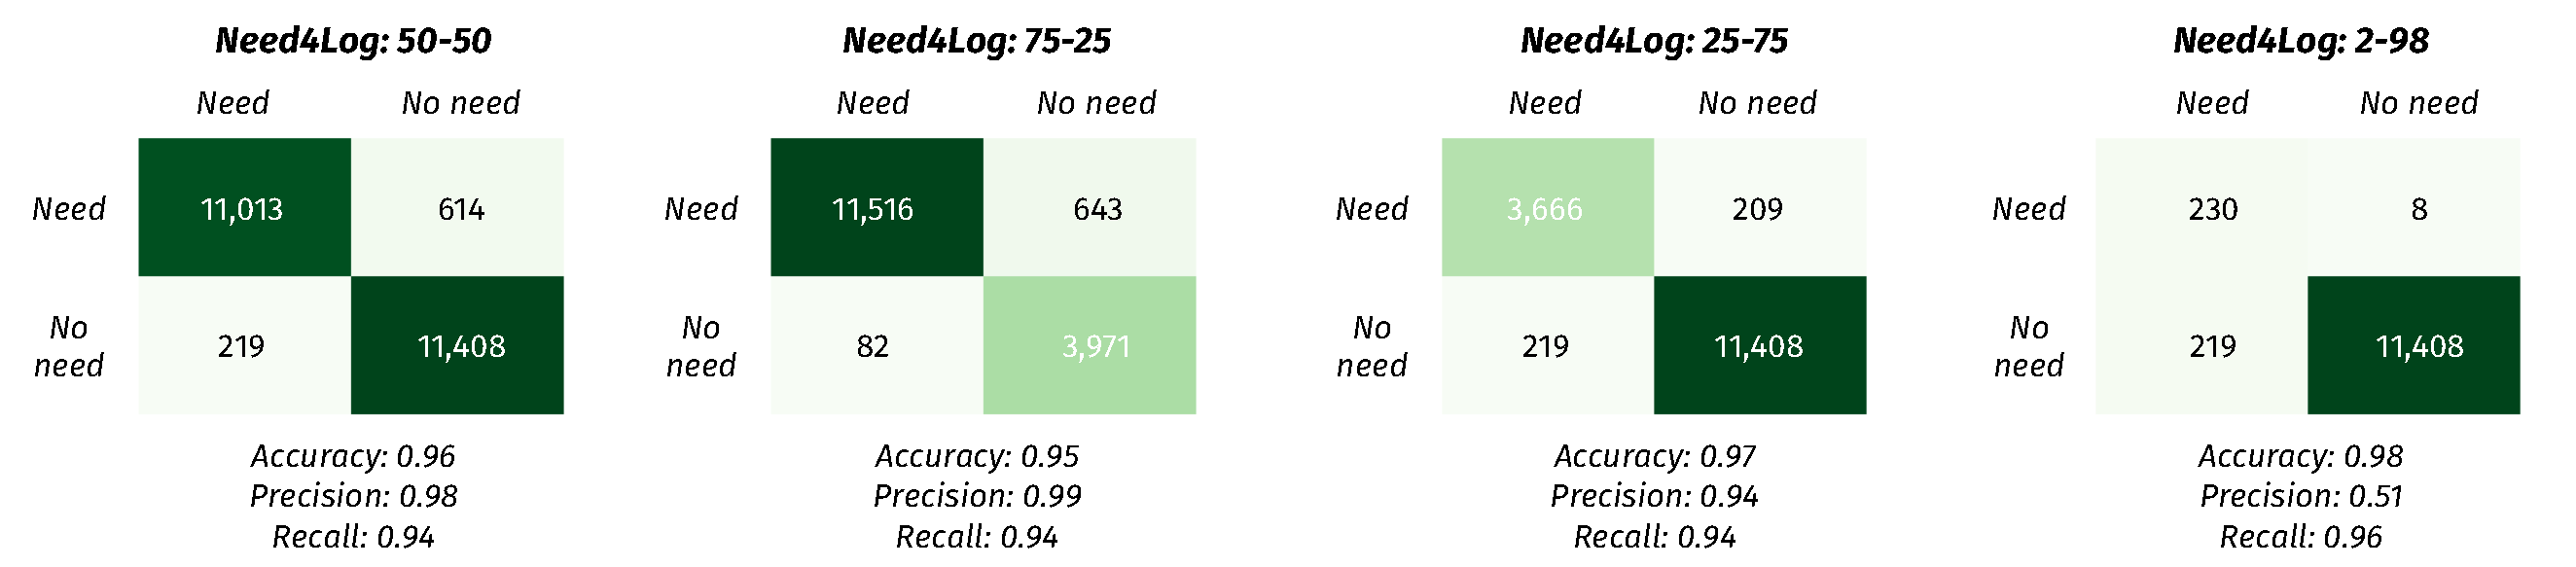
\includegraphics[width=\textwidth]{img/RQ3-CM.pdf}
	\caption{Results achieved by LEONID when deciding whether log statements are needed or not in \java methods. For each test-set (\tabref{tab:ds-summary-2}), accuracy, precision and recall are reported.}
\end{figure*}



%complementarity
%Shared:  72.05602393255371
%Only LEONID:  14.781071525700298
%Only LANCE:  13.162904541745988

